
\section{Online Analytic Processing (OLAP)}

%\begin{breakbox}
%\boxtitle{Spezielle OLAP Operationen:}
%\newline Slice-and-dice:
%\begin{center}
%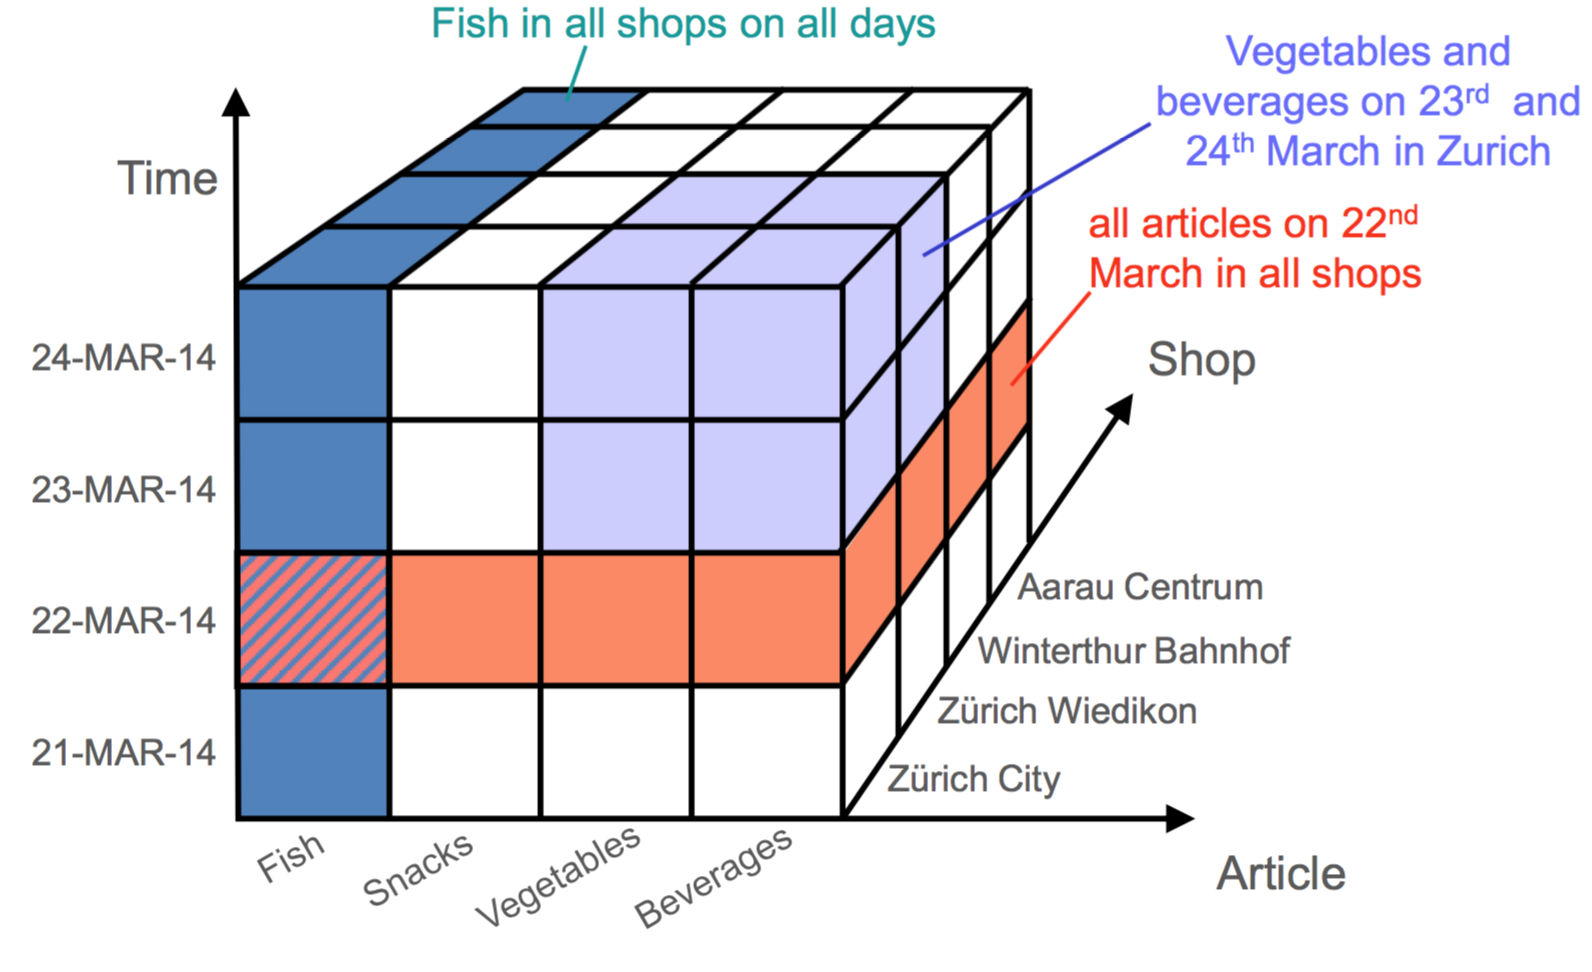
\includegraphics[width=.1\textwidth]{slides_images/slice_and_dice.png}
%\end{center}
%Drill-down:
%\begin{center}
%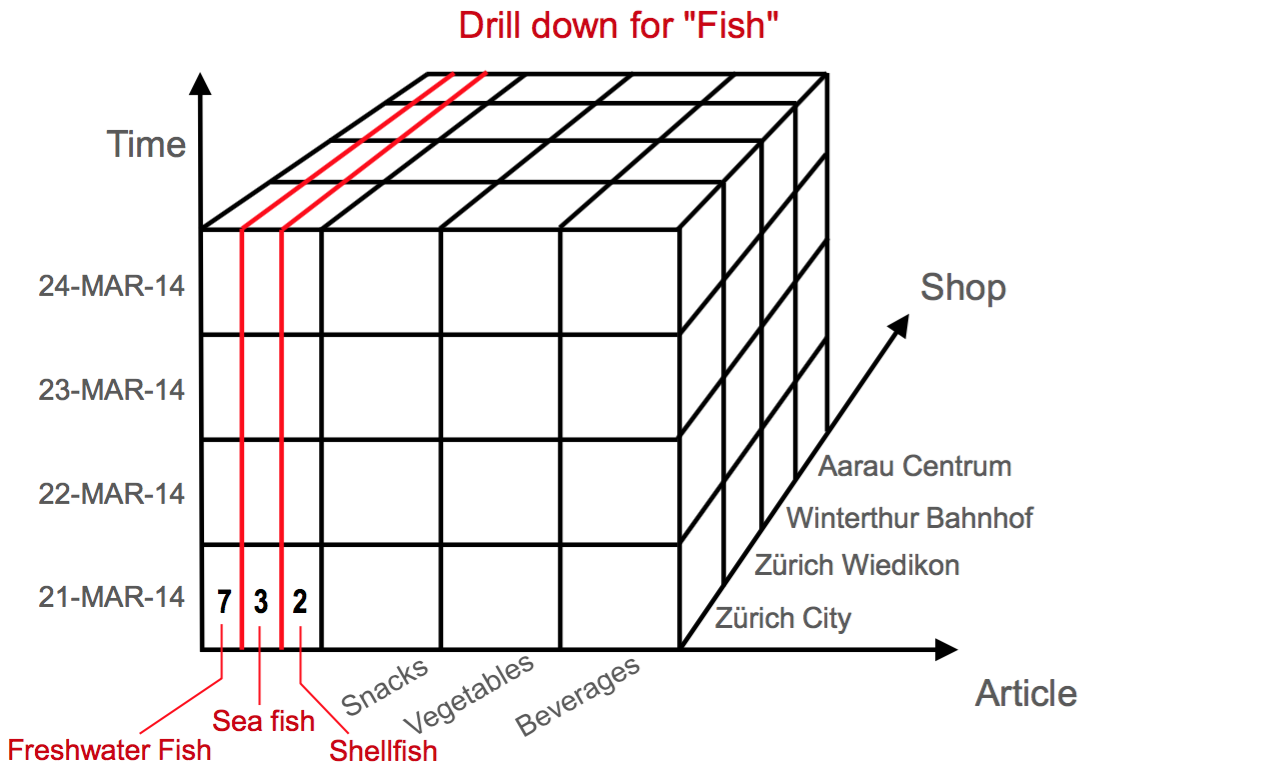
\includegraphics[width=.1\textwidth]{slides_images/drill_down.png}
%\end{center}
%Roll-up:
%\begin{center}
%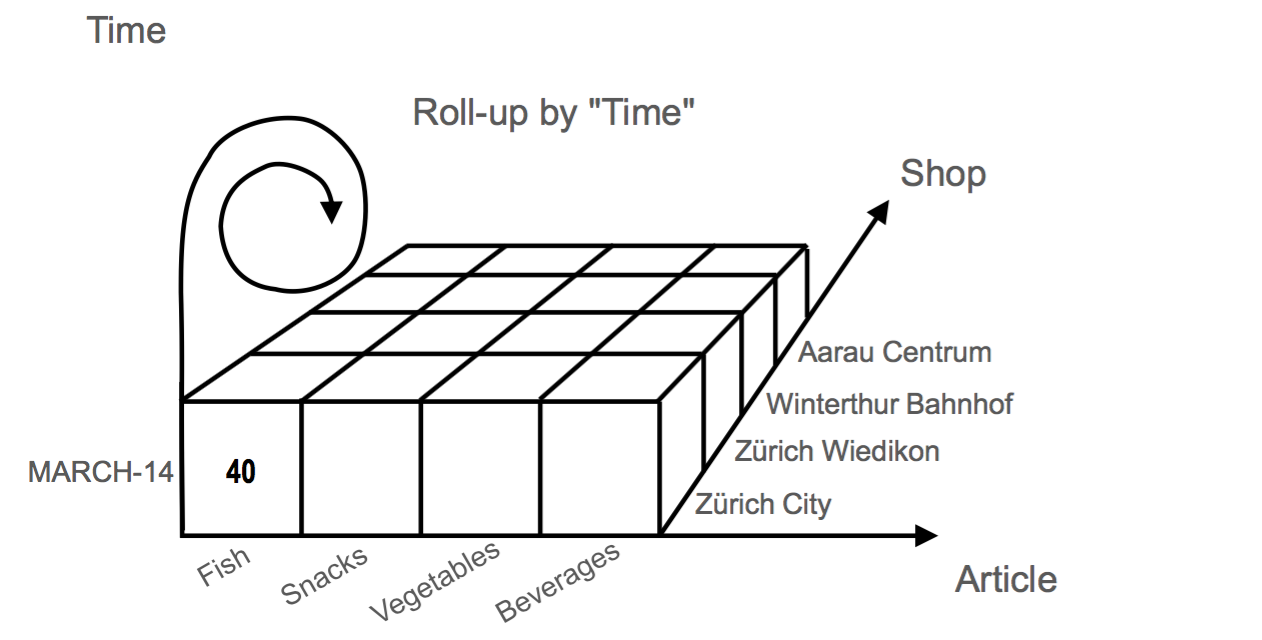
\includegraphics[width=.1\textwidth]{slides_images/roll_up.png}
%\end{center}
%\end{breakbox}

\begin{breakbox}
\boxtitle{CUBE:}
\sql{sql_code/cube.sql}
Merke:
\begin{itemize}
	\item Bei n Dimensionen ergibt CUBE $2^n$ Einträge.
	\item Das Resultat des CUBE Operators enthält alle Einträge zur Erstellung von cross tabulations:
\end{itemize}
\begin{center}
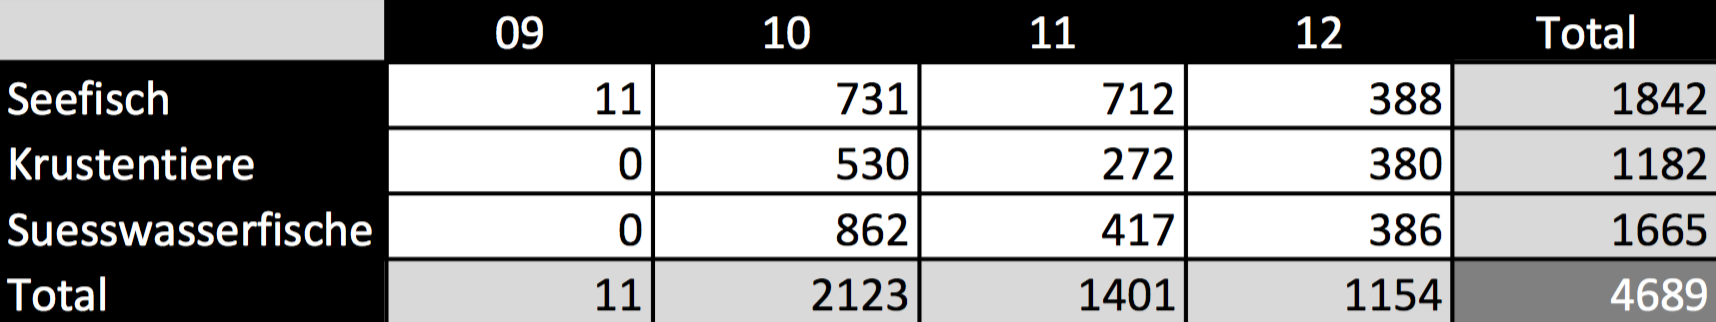
\includegraphics[width=.15\textwidth]{slides_images/cross_tabulation.png}
\end{center}
\end{breakbox}

\begin{breakbox}
\boxtitle{ROLLUP:}
\sql{sql_code/rollup.sql}
Merke:
\begin{itemize}
	\item Die Dimensionen werden von rechts her gruppiert.
	\item GROUPING kann verwendet werden, um zu sehen, welche Records gruppiert worden sind.
\end{itemize}
\end{breakbox}

\begin{breakbox}
\boxtitle{Bi-Temporale Tabellen:}
\newline Update:
\begin{center}
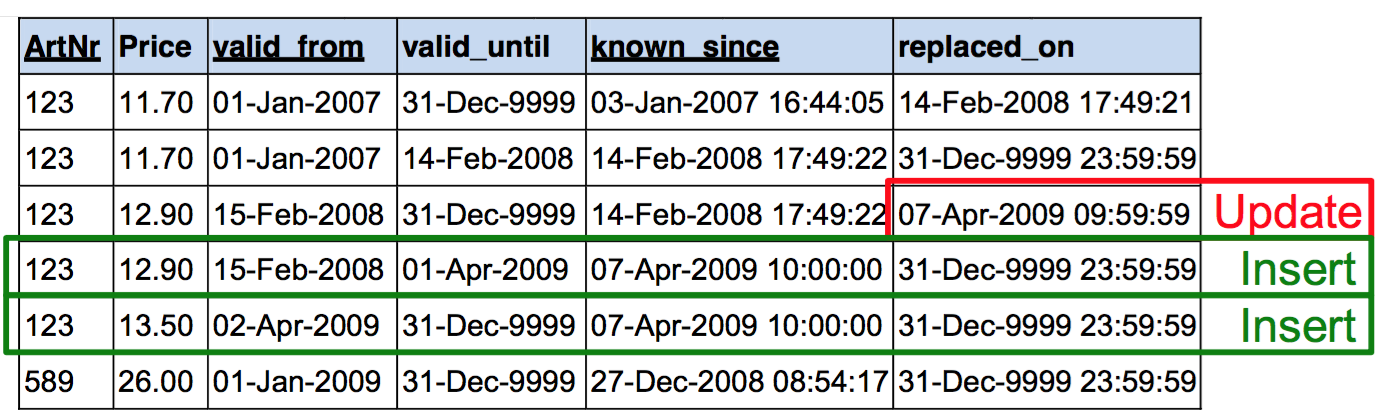
\includegraphics[width=.15\textwidth]{slides_images/bi_temporal_update.png}
\end{center}
Merke:
\begin{itemize}
	\item Der valid\_from und der known\_since Eintrag werden zusammen mit der ArtNr zum Primary Key, damit Einträge eindeutig bleiben.
\end{itemize}
\end{breakbox}

%\begin{breakbox}
%\boxtitle{CREATE Star Schema:}
%\sql{sql_code/create_star_schema.sql}
%\end{breakbox}
